\documentclass[a4paper, 12pt]{article}
\usepackage{listings} 
\usepackage{xcolor}
\usepackage{mdframed}
\usepackage{graphicx}
\usepackage{pgfplots}
\usepackage{float}
\usepackage{mathtools}

%% Custom FSM's
\usepackage{tikz}
\usetikzlibrary{automata, positioning, arrows}
\tikzset{thick, ->, >=stealth', node distance=6cm, every state/.style={thick, fill=gray!10}, initial text=$ $}

%% Macros for logic timing diagrams
\newcounter{wavenum}
\setlength{\unitlength}{1cm}
% advance clock one cycle, not to be called directly
\newcommand*{\clki}{
  \draw (t_cur) -- ++(0,.3) -- ++(.5,0) -- ++(0,-.6) -- ++(.5,0) -- ++(0,.3)
    node[time] (t_cur) {};
}
\newcommand*{\bitvector}[3]{
  \draw[fill=#3] (t_cur) -- ++( .1, .3) -- ++(#2-.2,0) -- ++(.1, -.3)
                         -- ++(-.1,-.3) -- ++(.2-#2,0) -- cycle;
  \path (t_cur) -- node[anchor=mid] {#1} ++(#2,0) node[time] (t_cur) {};
}
% \known{val}{length}
\newcommand*{\known}[2]{
    \bitvector{#1}{#2}{white}
}
% \unknown{length}
\newcommand*{\unknown}[2][XXX]{
    \bitvector{#1}{#2}{black!20}
}
% \bit{1 or 0}{length}
\newcommand*{\bit}[2]{
  \draw (t_cur) -- ++(0,.6*#1-.3) -- ++(#2,0) -- ++(0,.3-.6*#1)
    node[time] (t_cur) {};
}
% \unknownbit{length}
\newcommand*{\unknownbit}[1]{
  \draw[ultra thick,black!50] (t_cur) -- ++(#1,0) node[time] (t_cur) {};
}
% \nextwave{name}
\newcommand{\nextwave}[1]{
  \path (0,\value{wavenum}) node[left] {#1} node[time] (t_cur) {};
  \addtocounter{wavenum}{-1}
}
% \clk{name}{period}
\newcommand{\clk}[2]{
    \nextwave{#1}
    \FPeval{\res}{(\wavewidth+1)/#2}
    \FPeval{\reshalf}{#2/2}
    \foreach \t in {1,2,...,\res}{
        \bit{\reshalf}{1}
        \bit{\reshalf}{0}
    }
}

% \begin{wave}[clkname]{num_waves}{clock_cycles}
\newenvironment{wave}[3][clk]{
  \begin{tikzpicture}[draw=black, yscale=.7,xscale=1]
    \tikzstyle{time}=[coordinate]
    \setlength{\unitlength}{1cm}
    \def\wavewidth{#3}
    \setcounter{wavenum}{0}
    \nextwave{#1}
    \foreach \t in {0,1,...,\wavewidth}{
      \draw[dotted] (t_cur) +(0,.5) node[above] {t=\t} -- ++(0,.4-#2);
      \clki
    }
}{\end{tikzpicture}}

% Specific Line Breaks
% See https://tex.stackexchange.com/questions/26174/ for details
\usepackage[british]{babel} 

% Page Margins
\usepackage[margin=1.00in]{geometry}

% Large, array-sized, ceiling and floor operators
\DeclarePairedDelimiter\ceil{\lceil}{\rceil}
\DeclarePairedDelimiter\floor{\lfloor}{\rfloor}
\definecolor{code-gray}{gray}{0.93}

% Beginning of Document
\begin{document}
% Title
\title{ECE 440 - Homework \#2}
\author{Collin Heist}
\date{\today}
\maketitle

% Table of Content and Listings
\pagenumbering{arabic}

% Beginning of Report
\section{Problem 1}
\begin{center}
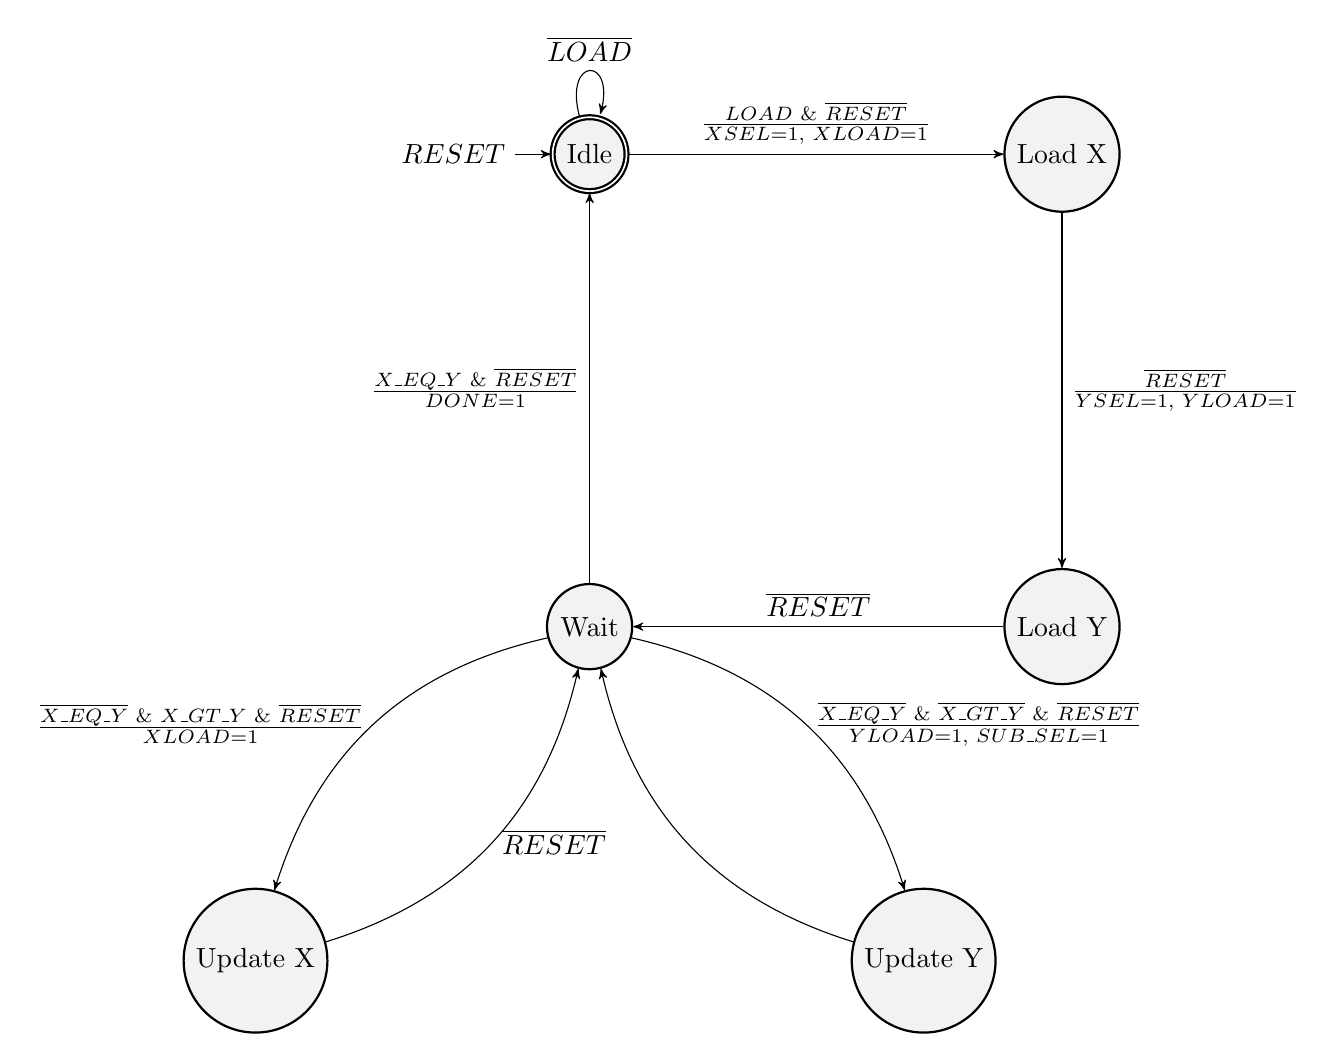
\begin{tikzpicture}[initial text=$RESET$]
	\node[state, initial, accepting] (Idle) {Idle};
	\node[state, right of=Idle] (Load X) {Load X};
	\node[state, below of=Load X] (Load Y) {Load Y};
	\node[state, left of=Load Y] (Wait) {Wait};
	\node[state, below left of=Wait] (Update X) {Update X};
	\node[state, below right of=Wait] (Update Y) {Update Y};
	
	\draw	(Idle) edge[loop above] node{$\overline{LOAD}$} (Idle)
				(Idle) edge[above] node{$\frac{LOAD \text{ \& }\overline{RESET}}{XSEL=1\text{, }XLOAD=1}$} (Load X)
				(Load X) edge[right] node{$\frac{\overline{RESET}}{YSEL=1\text{, }YLOAD=1}$} (Load Y)
				(Load Y) edge[above] node{$\overline{RESET}$} (Wait)
				(Wait) edge[bend right, left] node{$\frac{\overline{X\_EQ\_Y}\text{ \& }X\_GT\_Y \text{ \& }\overline{RESET}}{XLOAD=1}$} (Update X)
				(Update X) edge[bend right, right] node{$\overline{RESET}$} (Wait)
				(Wait) edge[bend left, right] node{$\frac{\overline{X\_EQ\_Y}\text{ \& }\overline{X\_GT\_Y}\text{ \& }\overline{RESET}}{YLOAD=1\text{, }SUB\_SEL=1}$} (Update Y)
				(Update Y) edge[bend left, left] node{} (Wait)
				(Wait) edge[left] node{$\frac{X\_EQ\_Y\text{ \& }\overline{RESET}}{DONE=1}$} (Idle);
\end{tikzpicture}
\end{center}

\newpage
\section{Problem 2}
\begin{center}
\begin{wave}[\textbf{Clock}]{17}{9}
	\nextwave{DIN[0:8]} \unknown[x]{1.7} \known{6}{0.6} \unknown[x]{0.4} \known{4}{0.6} \unknown[x]{6.7}
	\nextwave{RESET} \bit{0}{10}
	\nextwave{LOAD} \bit{0}{0.7} \bit{1}{0.6} \bit{0}{10-0.7-0.6}
	\nextwave{RESULT} \unknown[x]{2} \known{6}{3} \known{2}{5}
	\nextwave{DONE} \bit{0}{8.3} \bit{1}{1} \bit{0}{0.7}
	\nextwave{STATE} \known{\tiny{Idle}}{1.3} \known{\tiny{Load X}}{1} \known{\tiny{Load Y}}{1} \known{\tiny{Wait}}{1} \known{\tiny{Up. X}}{1} \known{\tiny{Wait}}{1} \known{\tiny{Up. Y}}{1} \known{\tiny{Wait}}{1} \known{\tiny{Idle}}{1.7}
	\nextwave{XSEL} \bit{0}{1.3} \bit{1}{1} \bit{0}{7.7}
	\nextwave{XLOAD} \bit{0}{1.3} \bit{1}{1} \bit{0}{2} \bit{1}{1} \bit{0}{4.7}
	\nextwave{YSEL} \bit{0}{2.3} \bit{1}{1} \bit{0}{6.7}
	\nextwave{YLOAD} \bit{0}{2.3} \bit{1}{1} \bit{0}{3} \bit{1}{1} \bit{0}{2.7}
	\nextwave{SUB\_SEL} \bit{0}{6.3} \bit{1}{1} \bit{0}{2.7}
	\nextwave{X\_EQ\_Y} \unknownbit{3} \bit{0}{4} \bit{1}{3}
	\nextwave{X\_GT\_Y} \unknownbit{3} \bit{1}{2} \bit{0}{5}
	\nextwave{X} \unknown[x]{2} \known{6}{3} \known{2}{5}
	\nextwave{Y} \unknown[x]{3} \known{4}{4} \known{2}{3}
	\nextwave{DIFF} \unknown[x]{3} \known{2}{2} \unknown[x]{1.3} \known{2}{0.7} \known{0}{3}
\end{wave}
\end{center}

\textit{Note: The temporary unknown value of the \textbf{DIFF} line is due to this being affected by the ALU being used. For that small period, $2-4$ is being computed - resulting in an n-bit 2's complement number.}

\section{Problem 3}
	\begin{mdframed}[backgroundcolor=code-gray, roundcorner=10pt,
								innerleftmargin=5, innertopmargin=5, innerbottommargin=5]	
	\begin{lstlisting}[language=Verilog, caption=Waveform Generation, tabsize=2, label={lst:init-hardware}]
	initial begin
		a = 0; b = 1; #3;
		a = 1; b = 0; #3;
		       b = 1; #2;
		a = 0;        #3;
		a = 1; b = 0; #1;
		a = 0;        #4;
	end
	\end{lstlisting}
	\end{mdframed}
		
\newpage
\section{Problem 4}
Scalar outputs N, Z, and V indicate when the alu's output is negative (2s complement), zero, or there is a twos complement overflow. 

	\begin{mdframed}[backgroundcolor=code-gray, roundcorner=10pt,
								innerleftmargin=5, innertopmargin=5, innerbottommargin=5]	
	\begin{lstlisting}[language=Verilog, caption=ALU Module, tabsize=2, label={lst:init-hardware}]
	module alu
		#(parameter width = 8)
		(input logic carry_in,
		input logic [1:0] fn,
		input logic [width-1:0] a, b,
		output logic carry_out, N, Z, V,
		output logic [width-1:0] result);
		
		// Make enumeration of logic operations
		typedef enum logic [1:0] {sADD, sAND, sOR, sXOR} alu_ops;
		
		// Determine if there is a carry-out
		logic [width:0] temp = {1'b0, a} + {1'b0, b};
		assign carry_out = temp[width];
		
		always_comb
		begin
			assign N = 0; assign Z = 0; assign V = 0;
			unique case(fn)
				sADD:
					begin
					assign result = a + b + carry_in;
					assign N = result[width-1];
					assign Z = (result == '0);
					assign V = (!a[width-1] & !b[width-1] &
						result[width-1]) | (a[width-1] & b[width-1] &
						!result[width-1);
					end
				sAND:	assign result = a & b;
				sOR:	assign result = a | b;
				sXOR:	assign result = a ^ b;
			endcase
		end		
	endmodule;
	\end{lstlisting}
	\end{mdframed}
	
	% Test bench
	
	\begin{mdframed}[backgroundcolor=code-gray, roundcorner=10pt,
								innerleftmargin=5, innertopmargin=5, innerbottommargin=5]	
	\begin{lstlisting}[language=Verilog, caption=ALU Testbench, tabsize=2, label={lst:init-hardware}]
		`timescale 1ns / 1ps
		module testbench;
			parameter width = 4;		
		
			logic carry_in, carry_out, N, Z, V;
			logic [1:0] fn;
			logic [width-1:0] a, b, result;
			
			alu dut(.*);
			
			initial begin
				carry_in = 0;
				fn = 2'b0;
				a = width'b0; b = width'b0;
				#100;	// Wait for global reset
				
				// Add (7) and (-7)
				fn = 2'b00;
				a = width'b0111; b = width'b1001; #3;
				if ((result == 'b0000) && (N == '0) &&
					(Z == '1) && (V == '0) && (carry_out == '0))
					$display("ADD test passed.");
					
				fn = 2'b01;
				a = width'b1110; b = width'b1100;
				if ((result == 'b1100) && (N == '0) && 
					(Z == '0) && (V == '0) && (carry_out == '0))
					$display("AND test passed.");
					
				fn = 2'b10;
				a = width'b0101; b = width'b1000;
				if ((result == 'b1101) && (N == '0) && 
					(Z == '0) && (V == '0) && (carry_out == '0))
					$display("OR test passed.");
					
				fn = 2'b11;
				a = width'b1101; b = width'b1011;
				if ((result == 'b0110) && (N == '0) && 
					(Z == '0) && (V == '0) && (carry_out == '0))
					$display("XOR test passed.");
			end
		endmodule
	\end{lstlisting}
	\end{mdframed}

\end{document}